\chapter{پهپاد دستیار آتشنشان}
\section{مقدمه}
\par
عرصه های طبیعی در سراسر جهان، ازجمله ایران، هر
ساله به علل گوناگون دچار حریق و آتش سوزی می شوند و 
خسارت های زیاد جانی، مالی، زیست محیطی و 
اکوسیستمی به کشورها وارد می کند.فقط در سال 1389
تعداد 210 مورد آتش سوزی در جنگل ها و مراتع شمال ایران 
رخ داده است 
\cite{eskandari2021fire}
. برای جلوگیری از گسترده شدن آتش سوزی بسیار اهمیت دارد که به موقع محل های آتش سوزی تشخیص داده  شوند و به سرعت خاموش شوند . استفاده از پهپاد های آتشنشان می تواند بسیار مفید واقع شود . 
\par
به علت اینکه آماده سازی جهت پرواز کوادکوپتر کوتاه است و همچنین در ختان جنگل مانعی برای حرکت این پرنده های کوچک به حساب نمی آیند  ، کوادکوپتر می تواند یکی از تجهیزاتی باشد که برای کنترل آتش سوزی ها به خصوص جنگل ها مورد استفاده قرار بگیرد . 
\section{طرح مسئله}
در 
\cite{kinaneva2019early} 
به ارائه یک پلتفرم با استفاده از دو پرنده هدایت پذیر پرداخته است ؛ یک پهپاد بال ثابت  که در ارتفاع متوسط (350 متر الی 5500 متر) پرواز می کند و وضعیت جنگل را بررسی می کند و در صورتی که آتش سوزی را تشخیص دهد آلارم هشدار را فعال می نماید . در این هنگام کواد کوپتری که در  ارتفاع پایین تری پرواز می کند به محل رفته و بررسی می کند که آیا این واقعا آن محل دچار آتش سوزی شده است یا خیر . علت استفاده از دو په پهپاد این طور عنوان شده است که در صورتی که از یک پهپاد بال ثابت که در ارتفاع بالاتر پرواز می کند  استفاده شود احتمال تشخیص اشتباه بالا می باشد واز طرفی استفاده از یک پهپاد در ارتفاع پایین موجب کاهش محدوه دید می شود .از جمله مزایای استفاده از پهپاد بال ثابت سرعت کروز بیشتر و ارتفاع پرواز بیشتر، راندمان پرواز بالا، استقامت و برد طولانی و مزیای کواد کوپتر انعطاف پذیری و توانایی فرود عبور از موانع  و فرود در محل هاکوچک می باشد . استفاده از چند پهپاد برای باز دید مناطق طبیعی و جنگل ها می تواند موجب بهبود عملکرد شود .
\begin{figure}[h]
	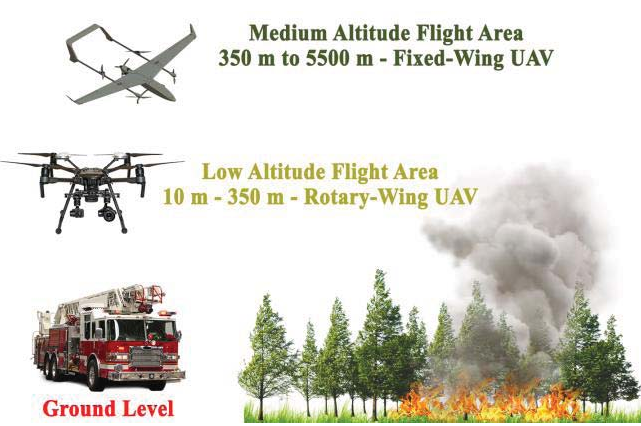
\includegraphics[scale=1]{fig quad1}
	\centering
	\caption{بخش اصلی  برای تشخیص زودهنگام آتش سوزی جنگل با استفاده از پهپادهای بال ثابت و بال چرخشی}
	\cite{kinaneva2019early}
	\label{fig1}
\end{figure} 
\begin{figure}[h]
	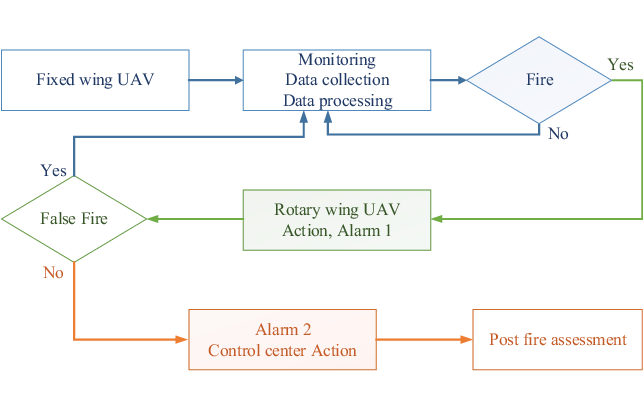
\includegraphics[scale=0.9]{quad2}
	\centering
	\caption{فلوچارت عملیات سیستم تشخیص حریق}
	\cite{kinaneva2019early}
	\label{fig2}
\end{figure} 
\section{مدل\lr{PEAS}} 
در این بخش به بررسی هوشمندی این سیستم دو پهپاده می پردازیم ؛ این سیستم را از نظر ویژگی های عملکرد ،  محیط ، عملگرها و حسگرها می سنجیم .
\subsection{اندازه گیری عمکرد} 
اندازه گیری عملکرد
\footnote{\lr{performance measure}}
برای این سیستم به این صورت است که با مصرف کمترین انرژی بتوان آتش سوزی ها را در کمترین زمان ممکن یافت . طبیعی است که اشتباه در تشخیص محل آتش سوزی باعث افزایش مصرف انرژی می باشد .
\subsection{محیط}
محیط در مورد این مثال آسمان  جنگل می شود . در حقیقت برای هر پهپاد ارتفاع پرواز آن هم اهمیت دارد . که برای پهپاد  بال ثابت 350 متر تا 5500 متر و برای پهپاد بال چرخان 10 متر تا 350 متر می باشد . 
\par 
محیط به صورت کامل رویت پذیر نمی باشد و رویت پذیر جزئی 
\footnote{\lr{partially observable environment}}
می باشد . هم چنین در مورد این محیط می توان گفت آتش سوزی در هر جایی می تواند رخ دهد و با یک احتمالی بنابرای محیط تصادفی
\footnote{\lr{stochastic environment}}
است و نیز با توجه به وجود دو پهپاد محیط چند کاربره
\footnote{\lr{multi agent}}
است . درعین حال پهپاد های دیگری هم می توانند مناطق دیگری را پوشش دهند و باعث شود که تعداد بسیار بیشتری پهپاد در محیط حضور داشته باشند که نیاز است با هم هماهنگ باشند . محیط پیوسته
\footnote{\lr{continuous environment}}
می باشد و پهپاد در هرکجا از محدوده ی حرکتی می توانند بروند .
محیط به صورت 
\lr{sequential}
 می باشد و هر حرکت پهپاد بر روی حرکات بعدی نیز موثر است .

\subsection{عملگر}
عملگر های پهپاد ها موتور های پره دار آن هاست برای پرواز و همین طور آلارمی که فعلا یا غیر فعال می کنند .
\subsection{حسگر}
این پرنده ها به وسیله ی دوربین هایی که دارند محیط را می بینند . این دوربین ها به صورت نوری و یا حرارتی می باشند . به وسیله یه شبکه عصبی تشخیص و لگوریتم های بینایی ماشین
\footnote{\lr{computer vision}}
محل دود یا آتش  میسر می شود .
\section{جمع بندی}
در این فصل به بررسی پهپاد های کمک آتشنشان پرداختیم و دیدیم که این پهپاد ها با استفاده از الگوریتم های بینایی ماشین به تشخیص محل های آتش سوزی می پردازند . هر یک از عمل هایی که انجام می دهند با توجه به 
\lr{rationality}
خود سعی دارند تا پاسخ مناسب بدهند . همچنین در 
\cite{kinaneva2019early}
این موضوع گفته شده است که برای بهتر شدن عملکرد این قابلیت در سیستم قرار داده شود که بتوانند پیش بینی کنند کدام ناحیه بیشتر در معرض آتش سوزی قرار دارد . به این ترتیب این پهپاد ها به صورت خودمختار و بدون کنترل انسان می توانند به کنترل و مهار آتش سوزی های طبیعت کمک کنند .
